\documentclass[a4paper]{article}
\usepackage[utf8]{inputenc} % accents xuten bé
\usepackage[T1]{fontenc} % també pels accents, meh
\usepackage[catalan]{babel} % idioma
\usepackage{titlesec} % per a canviar format dels títols
\usepackage{titling} % per a poder definir \subtitle
%\usepackage[none]{hyphenat} % no separa paraules
\usepackage{mathtools} % millor que amsmath (opcions de notació mates)
\usepackage{amsfonts} % segurament per definir = amb coses dalt
\usepackage{cases} % per poder fer les típiques definicions per parts de funcions amb corxets
\usepackage{blindtext} % textos de prova, tipus loremipsum
\usepackage{enumitem} % llistes
\usepackage{geometry} % per controlar els marges
\usepackage{indentfirst} % per controlar la indentació de la primera línia de cada paràgraf
\usepackage{physics} % sobretot, derivades (parcials)
\usepackage{xcolor} % colors
\usepackage{float} % per controlar posicions de flotants (imatges i taules)
\usepackage{hyperref}
\usepackage{multirow}
\usepackage[per-mode=symbol]{siunitx}
\usepackage{graphicx}
\usepackage{caption}
\usepackage{subcaption}
%\usepackage{biblatex}
%\usepackage[
%backend=biber,
%style=alphabetic,
%citestyle=authoryear
%]{biblatex}

\usepackage{graphicx} % alguna cosa per a imatges
\graphicspath{ {./images/} }

% Que la primera línia no estigui indentada
\setlength{\parskip}{\baselineskip}
\setlength{\parindent}{0cm}

%\titlelabel{\llap{\thetitle\quad}} % No indentació dels títols

%Marges
%\hoffset = 0in
%\oddsidemargin = 13pt
%\textwidth = 427pt

%Comandes útils
\newcommand\eqdef{\mathrel{\overset{\makebox[0pt]{\mbox{\normalfont\tiny\sffamily def}}}{=}}}
\newcommand\eqimp{\mathrel{\overset{\makebox[0pt]{\mbox{\normalfont\tiny\sffamily imp}}}{=}}}
\newcommand\eqtext[1]{\mathrel{\overset{\makebox[0pt]{\mbox{\normalfont\tiny\sffamily {#1}}}}{=}}}
\renewcommand\vnabla{\vec{\nabla}}
\newcommand\vecv{\vec{v}}
\newcommand{\vvec}[1]{\vec{\vec{#1}}}
\newcommand\vecdot[1]{\dot{\vec{#1}}}
\newcommand\redtext[1]{\textcolor{red}{#1}}
\newcommand{\ten}[2]{\ensuremath{{#1}\times 10^{#2}}}
\DeclareMathOperator\arctanh{arctanh}

% definició de \subtitle
\newcommand{\subtitle}[1]{%
  \posttitle{%
    \par\end{center}
    \begin{center}\large#1\end{center}
    \vskip0.5em}%
}

% Format dels títols
\titleformat*{\section}{\Large\bfseries}
\titleformat*{\subsection}{\bfseries}

\captionsetup{
    width=\textwidth, % width of caption is 90% of current textwidth
    labelfont=bf,        % the label, e.g. figure 12, is bold
    font=small,          % the whole caption text (label + content) is small
%    format=hang,         % no caption text under the label
}

% Si funcionés, algun format de pàgina
%\pagestyle{fancy}
%\fancyhf{}
%\rhead{Share\LaTeX}
%\lhead{Guides and tutorials}
%\rfoot{Page \thepage}

% AND HERE WE GO

\title{\textbf{Simulació 2D del Model d'Ising}}
\subtitle{\scshape{Fenòmens col·lectius i transicions de fase}}
\author{Ivan Alsina Ferrer}
\date{December 2019}

\begin{document}

\maketitle

\section{Introducció}

\section{Evolució de magnetitzacions i temperatures}

L'algorisme de Metropolis accepta els canvis en la configuració que comporten una variació d'energia negativa, i n'accepta aquells que comporten una variació d'energia positiva amb una probabilitat que decau exponencialment amb el valor d'aquesta variació, amb la qual cosa s'ajusta a la naturalesa probabilística de les fluctuacions en el sistema. És per aquest motiu que, tot i no haver definit una dinàmica pròpia del sistema, podem argumentar que les iteracions Montecarlo en la simulació donen una noció de l'evolució temporal d'un sistema que, partint d'una configuració inicial aleatòria (en el nostre cas, determinada per la seed que fem servir), es veuen sotmesos a una temperatura donada.


\begin{figure}[H]
    \centering
    \begin{subfigure}{.8\textwidth}
        \centering
        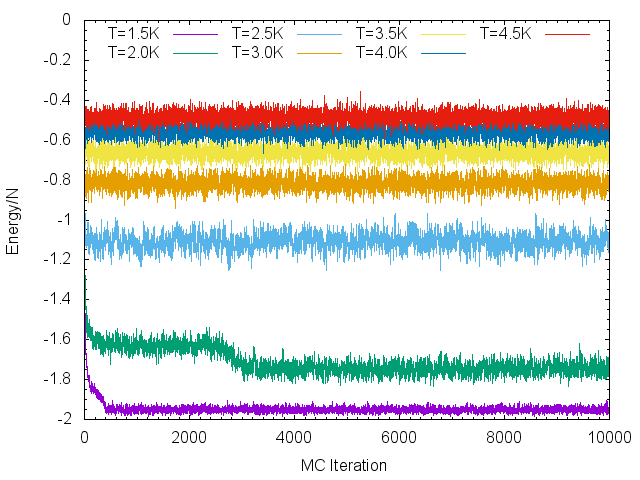
\includegraphics[width=0.8\textwidth]{SIM-L-060-energy-EVO.png}
        \label{evo_ene}
    \end{subfigure}
    \begin{subfigure}{.8\textwidth}
        \centering
        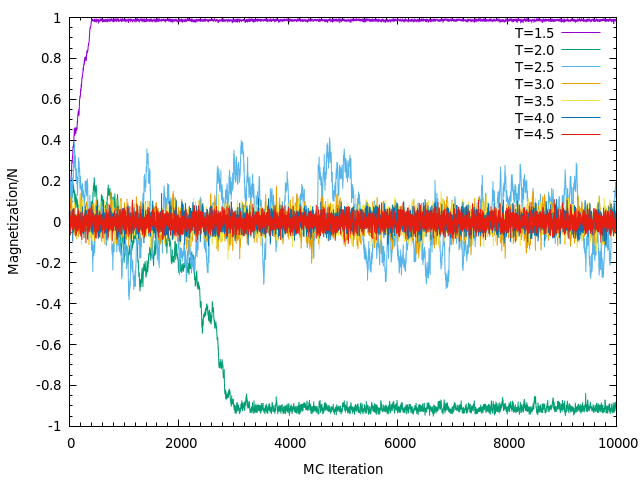
\includegraphics[width=0.8\textwidth]{SIM-L-060-magnetiz-EVO.png}
        \label{evo_mag}
    \end{subfigure}
    \caption{Evolució de les energies per partícula (a dalt) i les magnetitzacions per partícula (a baix) al llarg de les iteracions Montecarlo, per a temperatures reduïdes $T^*$ en el rang 1.5 a 4.5, en un sistema quadrat de $L=60$ spins de costat.}
\label{evo}
\end{figure}

Tal com veiem a la figura \ref{evo_ene}, per a temperatures baixes l'energia  del sistema convergeix ràpidament a 

\section{Magnituds termodinàmiques}

\section{Efecte de variar la mida}

\section{Temperatura crítica. Límit termodinàmic}

\section{Exponents crítics}

\section{Finite size scaling}

\section{Conclusions}

\section{Referències}

\end{document}

